\documentclass{ximera}

%\usepackage{todonotes}

\newcommand{\todo}{}

\usepackage{esint} % for \oiint
\graphicspath{
{./}
{functionsOfSeveralVariables/}
{normalVectors/}
{lagrangeMultipliers/}
{vectorFields/}
{greensTheorem/}
{shapeOfThingsToCome/}
}


\usepackage{tkz-euclide}
\tikzset{>=stealth} %% cool arrow head
\tikzset{shorten <>/.style={ shorten >=#1, shorten <=#1 } } %% allows shorter vectors

\usetikzlibrary{backgrounds} %% for boxes around graphs
\usetikzlibrary{shapes,positioning}  %% Clouds and stars
\usetikzlibrary{matrix} %% for matrix
\usepgfplotslibrary{polar} %% for polar plots
\usetkzobj{all}
\usepackage[makeroom]{cancel} %% for strike outs
%\usepackage{mathtools} %% for pretty underbrace % Breaks Ximera
\usepackage{multicol}
\usepackage{pgffor} %% required for integral for loops


%% http://tex.stackexchange.com/questions/66490/drawing-a-tikz-arc-specifying-the-center
%% Draws beach ball
\tikzset{pics/carc/.style args={#1:#2:#3}{code={\draw[pic actions] (#1:#3) arc(#1:#2:#3);}}}



\usepackage{array}
\setlength{\extrarowheight}{+.1cm}   
\newdimen\digitwidth
\settowidth\digitwidth{9}
\def\divrule#1#2{
\noalign{\moveright#1\digitwidth
\vbox{\hrule width#2\digitwidth}}}





\newcommand{\RR}{\mathbb R}
\newcommand{\R}{\mathbb R}
\newcommand{\N}{\mathbb N}
\newcommand{\Z}{\mathbb Z}

%\newcommand{\sage}{\textsf{SageMath}}


%\renewcommand{\d}{\,d\!}
\renewcommand{\d}{\mathop{}\!d}
\newcommand{\dd}[2][]{\frac{\d #1}{\d #2}}
\newcommand{\pp}[2][]{\frac{\partial #1}{\partial #2}}
\renewcommand{\l}{\ell}
\newcommand{\ddx}{\frac{d}{\d x}}

\newcommand{\zeroOverZero}{\ensuremath{\boldsymbol{\tfrac{0}{0}}}}
\newcommand{\inftyOverInfty}{\ensuremath{\boldsymbol{\tfrac{\infty}{\infty}}}}
\newcommand{\zeroOverInfty}{\ensuremath{\boldsymbol{\tfrac{0}{\infty}}}}
\newcommand{\zeroTimesInfty}{\ensuremath{\small\boldsymbol{0\cdot \infty}}}
\newcommand{\inftyMinusInfty}{\ensuremath{\small\boldsymbol{\infty - \infty}}}
\newcommand{\oneToInfty}{\ensuremath{\boldsymbol{1^\infty}}}
\newcommand{\zeroToZero}{\ensuremath{\boldsymbol{0^0}}}
\newcommand{\inftyToZero}{\ensuremath{\boldsymbol{\infty^0}}}



\newcommand{\numOverZero}{\ensuremath{\boldsymbol{\tfrac{\#}{0}}}}
\newcommand{\dfn}{\textbf}
%\newcommand{\unit}{\,\mathrm}
\newcommand{\unit}{\mathop{}\!\mathrm}
\newcommand{\eval}[1]{\bigg[ #1 \bigg]}
\newcommand{\seq}[1]{\left( #1 \right)}
\renewcommand{\epsilon}{\varepsilon}
\renewcommand{\phi}{\varphi}


\renewcommand{\iff}{\Leftrightarrow}

\DeclareMathOperator{\arccot}{arccot}
\DeclareMathOperator{\arcsec}{arcsec}
\DeclareMathOperator{\arccsc}{arccsc}
\DeclareMathOperator{\si}{Si}
\DeclareMathOperator{\proj}{\vec{proj}}
\DeclareMathOperator{\scal}{scal}
\DeclareMathOperator{\sign}{sign}


%% \newcommand{\tightoverset}[2]{% for arrow vec
%%   \mathop{#2}\limits^{\vbox to -.5ex{\kern-0.75ex\hbox{$#1$}\vss}}}
\newcommand{\arrowvec}{\overrightarrow}
%\renewcommand{\vec}[1]{\arrowvec{\mathbf{#1}}}
\renewcommand{\vec}{\mathbf}
\newcommand{\veci}{{\boldsymbol{\hat{\imath}}}}
\newcommand{\vecj}{{\boldsymbol{\hat{\jmath}}}}
\newcommand{\veck}{{\boldsymbol{\hat{k}}}}
\newcommand{\vecl}{\boldsymbol{\l}}
\newcommand{\uvec}[1]{\mathbf{\hat{#1}}}
\newcommand{\utan}{\mathbf{\hat{t}}}
\newcommand{\unormal}{\mathbf{\hat{n}}}
\newcommand{\ubinormal}{\mathbf{\hat{b}}}

\newcommand{\dotp}{\bullet}
\newcommand{\cross}{\boldsymbol\times}
\newcommand{\grad}{\boldsymbol\nabla}
\newcommand{\divergence}{\grad\dotp}
\newcommand{\curl}{\grad\cross}
%\DeclareMathOperator{\divergence}{divergence}
%\DeclareMathOperator{\curl}[1]{\grad\cross #1}
\newcommand{\lto}{\mathop{\longrightarrow\,}\limits}

\renewcommand{\bar}{\overline}

\colorlet{textColor}{black} 
\colorlet{background}{white}
\colorlet{penColor}{blue!50!black} % Color of a curve in a plot
\colorlet{penColor2}{red!50!black}% Color of a curve in a plot
\colorlet{penColor3}{red!50!blue} % Color of a curve in a plot
\colorlet{penColor4}{green!50!black} % Color of a curve in a plot
\colorlet{penColor5}{orange!80!black} % Color of a curve in a plot
\colorlet{penColor6}{yellow!70!black} % Color of a curve in a plot
\colorlet{fill1}{penColor!20} % Color of fill in a plot
\colorlet{fill2}{penColor2!20} % Color of fill in a plot
\colorlet{fillp}{fill1} % Color of positive area
\colorlet{filln}{penColor2!20} % Color of negative area
\colorlet{fill3}{penColor3!20} % Fill
\colorlet{fill4}{penColor4!20} % Fill
\colorlet{fill5}{penColor5!20} % Fill
\colorlet{gridColor}{gray!50} % Color of grid in a plot

\newcommand{\surfaceColor}{violet}
\newcommand{\surfaceColorTwo}{redyellow}
\newcommand{\sliceColor}{greenyellow}




\pgfmathdeclarefunction{gauss}{2}{% gives gaussian
  \pgfmathparse{1/(#2*sqrt(2*pi))*exp(-((x-#1)^2)/(2*#2^2))}%
}


%%%%%%%%%%%%%
%% Vectors
%%%%%%%%%%%%%

%% Simple horiz vectors
\renewcommand{\vector}[1]{\left\langle #1\right\rangle}


%% %% Complex Horiz Vectors with angle brackets
%% \makeatletter
%% \renewcommand{\vector}[2][ , ]{\left\langle%
%%   \def\nextitem{\def\nextitem{#1}}%
%%   \@for \el:=#2\do{\nextitem\el}\right\rangle%
%% }
%% \makeatother

%% %% Vertical Vectors
%% \def\vector#1{\begin{bmatrix}\vecListA#1,,\end{bmatrix}}
%% \def\vecListA#1,{\if,#1,\else #1\cr \expandafter \vecListA \fi}

%%%%%%%%%%%%%
%% End of vectors
%%%%%%%%%%%%%

%\newcommand{\fullwidth}{}
%\newcommand{\normalwidth}{}



%% makes a snazzy t-chart for evaluating functions
%\newenvironment{tchart}{\rowcolors{2}{}{background!90!textColor}\array}{\endarray}

%%This is to help with formatting on future title pages.
\newenvironment{sectionOutcomes}{}{} 



%% Flowchart stuff
%\tikzstyle{startstop} = [rectangle, rounded corners, minimum width=3cm, minimum height=1cm,text centered, draw=black]
%\tikzstyle{question} = [rectangle, minimum width=3cm, minimum height=1cm, text centered, draw=black]
%\tikzstyle{decision} = [trapezium, trapezium left angle=70, trapezium right angle=110, minimum width=3cm, minimum height=1cm, text centered, draw=black]
%\tikzstyle{question} = [rectangle, rounded corners, minimum width=3cm, minimum height=1cm,text centered, draw=black]
%\tikzstyle{process} = [rectangle, minimum width=3cm, minimum height=1cm, text centered, draw=black]
%\tikzstyle{decision} = [trapezium, trapezium left angle=70, trapezium right angle=110, minimum width=3cm, minimum height=1cm, text centered, draw=black]

\title{Practice Quiz}

\begin{document}
\begin{abstract}
Answer the questions honestly to assess your own abilities. This survey will not be graded. It can be used for you to determine your own strengths and weaknesses.
\end{abstract}
\maketitle

\begin{problem} 
    Would you be able to use the graph of a function to find the value of $f(2)$?
    
    \begin{center} 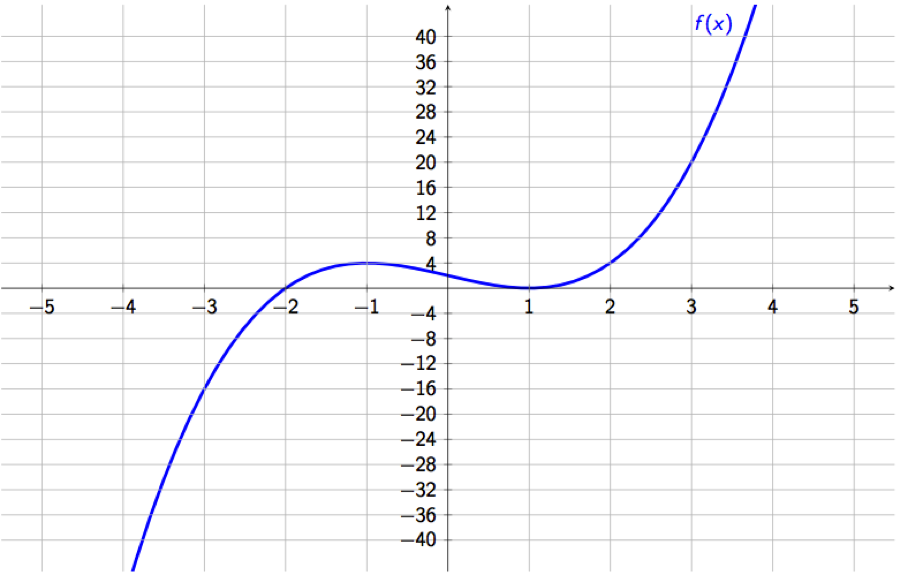
\includegraphics[scale = 0.7]{Graphing1.png} \end{center}
  \begin{multipleChoice}
      \choice[correct]{Yes, I could find $f(2)$.}
      \choice[correct]{Yes, but I would need to review some resources first.}
      \choice[correct]{No, I would need to learn/relearn how to do this.}
      \choice[correct]{I don't know.}
      \choice[correct]{I don't want to answer this question right now.}
  \end{multipleChoice}
\end{problem}

\begin{problem} 
    Could you factor the following polynomial?
    $$x^2 + 9x -36$$
  \begin{multipleChoice}
      \choice[correct]{Yes, I can factor this polynomial.}
      \choice[correct]{Yes, but I would need to review some resources first.}
      \choice[correct]{No, I would need to learn/relearn how to factor.}
      \choice[correct]{I don't know.}
      \choice[correct]{I don't want to answer this question right now.}
  \end{multipleChoice}
\end{problem}

\begin{problem} 
    Could you find the solutions to this equality?
    $$2x^2 - 4$$
  \begin{multipleChoice}
      \choice[correct]{Yes, I can factor this polynomial.}
      \choice[correct]{Yes, but I would need to review some resources first.}
      \choice[correct]{No, I would need to learn/relearn how to factor.}
      \choice[correct]{I don't know.}
      \choice[correct]{I don't want to answer this question right now.}
  \end{multipleChoice}
\end{problem}
        

\begin{problem}
  Which of the following approximate the slope of the ``zoomed line''? Select all that are correct.
  \begin{selectAll}
    \choice{$\frac{(f(a)+h) - f(a)}{(a+h)-a}$}
    \choice[correct]{$\frac{f(a+h) - f(a)}{(a+h)-a}$}
    \choice{$\frac{(f(a)-h) - f(a)}{(a-h)-a}$}
    \choice[correct]{$\frac{f(a-h) - f(a)}{(a-h)-a}$}
    \choice{$\frac{f(a) - (f(a)+h)}{a-(a+h)}$}
    \choice[correct]{$\frac{f(a) - f(a+h)}{a-(a+h)}$}
    \choice{$\frac{f(a) - (f(a)-h)}{a-(a-h)}$}
    \choice[correct]{$\frac{f(a) - f(a-h)}{a-(a-h)}$}
  \end{selectAll}
\end{problem}

\begin{problem}
   Let $f(x) = 3x-1$.  Zoom in on the curve around $a = -2$ so that $h
   = 0.1$.  Use one of the formulations in the problem above to
   approximate the slope of the curve.  The slope of the curve at $a =
   -2$ is approximately\dots \begin{prompt}$\answer{3}$\end{prompt}
\end{problem}

\begin{problem}
   Repeat the previous problem for $f(x) = x^2 - 1$, $a = 0$, and $h =
   0.2$.  Choose a formulation that will give you a positive answer
   for the slope.  The (positive) slope of the curve at $a = 0$ is
   approximately\dots\begin{prompt} $\answer{0.2}$\end{prompt}
\end{problem}


\begin{problem}
   Zoom in on the curve $f(x) = x^2 - 1$ near $x=0$ again.  By looking
   at the graph, what is your best guess for the actual slope of the
   curve at zero?
   \begin{multipleChoice}
     \choice{impossible to say}
     \choice[correct]{zero}
     \choice{one}
     \choice{infinity}
   \end{multipleChoice}
\end{problem}

%%% \begin{xarmaBoost}
%%   Write down at least \textbf{five} questions for this lecture. After
%%   you have your questions, label them as ``Level 1,'' ``Level 2,'' or
%%   ``Level 3'' where:
%% \begin{description}
%% \item[Level 1] Means you know the answer, or know exactly how to do
%%   this problem.
%% \item[Level 2] Means you think you know how to do the problem.
%% \item[Level 3] Means you have no idea how to do the problem.
%% \end{description}
%% \begin{freeResponse}
%% \end{freeResponse}
%% \end{xarmaBoost}



\end{document}
